\section{Software Quality Metrics}
Citat fra Troels: \textit{''Hvad kan man finde ud af om sit program, uden at køre det? Denne disciplin kaldes Static Analysis, og kan give feedback til programmøren, der er ligeså værdifuld som en faktisk test.''}\\

Statisk analyse kan bruges til: 

\begin{enumerate}
	\item Give \textit{quality measures}.
	\item Gennemtvinge \textit{code style and discipline}.
	\item Finde \textit{possible errors}.
\end{enumerate}

\subsection{Værktøjer} til formålet har vi nogle værktøjer.

\subsubsection{FxCop}
Statisk analyseværktøj, udviklet af Microsoft til Visual Studio. Lavet for at øge performance, sikkerhed og design.

\subsubsection{Compilers}
Compileren er et eksempel på et Statisk analyseværktøj. Alle moderne compilere viser advarseler og lignende for koden, nogle vigtige, andre not so much.

\subsubsection{ReSharper}
Finder også fejl, som ikke nødvendigvis er kritiske. F.eks informerer den om inkonsekvent navngivning, ikke initialiserede variabler og helt ubrugte variabler.

\subsection{Quantitative code analysis}
Aka: Software Metrics. Bruges til at beskrive: 

\begin{itemize}
	\item Microsoft Maintainability index.
	\item Cyclomatic complexity (se afsnit~\ref{sec:cyclomatic}).
	\item Lines of code per function/module.
\end{itemize}

\subsubsection{Maintainability}
Et index som beskriver hvor holdbar og effektiv ens kode er. Samt hvor let den er at vedligeholde. Indexet går fra 0-100, hvor 100 er bedst.

\def\arraystretch{1.5}%  1 is the default, change whatever you need
\begin{table}[H]
	\centering
	\begin{tabular}{|c|l|}
		\hline
		\hspace{2cm} \cellcolor{green}& 20-100\\
		\hline
		\cellcolor{yellow}& 10-19\\
		\hline
		\cellcolor{red}& 0-9\\
		\hline
	\end{tabular}
	\caption{Maintainability index score.}
\end{table}

\subsubsection{Lines of code}
Angiver antallet af \textit{intermediate language}\todo{hvorfor IL?} linjer i koden, altså \textbf{ikke} linjer i source koden. Bruges til at indikere om en metode laver for meget og skal deles op i flere mindre methoder.

\subsubsection{Class coupling}
Beskriver koblingen mellem klasser. Findes ved at kigge på parametre, returtyper, baseklasser, og interface-inplementeringer.

\subsubsection{Depth of inheritance}
Angiver hvor mange klasser, der 'hænger' sammen i klassernes arveheiraki. Jo dybere et arveheiraki, desto svære at finde ud af hvor klasserne er defineret. Derved sværere at vedligeholde.

\subsubsection{Cyclomatic Complexity}\label{sec:cyclomatic}
Bruges til at beskrive kompleksiteten i et program. Det er et kvantitativt mål for antallet af lineære uafhængige vejen gemmet programmets source code.

\begin{figure}[H]
	\centering
	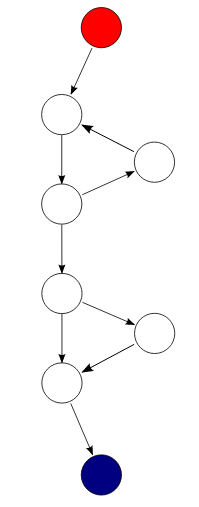
\includegraphics[width=0.8\linewidth]{figs/cyclomatic}
	\caption{Grafisk fremstiling af den cyclomatiske complexity i code listing~\ref{code:cyclomatic}.}
	\label{fig:cyclomatic}
\end{figure}

\begin{lstlisting}[caption=Kode for eksempel vist på figur~\ref{fig:cyclomatic}.,label=code:cyclomatic]
public void Method()
{
	while(Condition1) 
		Action1();		
	if(Condition2) 
		Action2();		
	Action3();	
	return;
}
\end{lstlisting}

Når man har en graf som vist på figur~\ref{fig:cyclomatic}, er følgende udtryk gældende: 

\begin{align}
E &= NumberOfEdges\\
N &= NumberOfNodes\\
P &= NumberOfConnectionComponents
\end{align}

\vskip.3cm

Med disse termer kan M (antallet af \textit{decision points}) findes sådan her:

\begin{align}
M &= E-N+2P\\
M&= 9-8+2*1=3
\end{align}




























